\documentclass{article}
\usepackage{graphicx} % Required for inserting images
\usepackage{amsmath}


\title{\textbf{MATRIX COMPUTATIONS: HOMEWORK 2}}  % Declares the document's title.
\author{Andre Theo,
Dejean Maxime,
Doat Damien,
Nouidei Safiya}  
\date{October 2024}
\setlength{\parindent}{0pt}
\begin{document}

\maketitle

\section{Exercise A: Krylov subspaces}
\subsection*{(A1)}
First of all, we have that 
\begin{align*}
    \mathcal{K}_{r}(A,b) &=span\{b, Ab, ..., A^{r-1}b\},\\
    \mathcal{K}_{s}(A,b) &=span\{b, Ab, ..., A^{s-1}b\}.
\end{align*}
So since $r\leq s$, we have that $\mathcal{K}_r(A,b) \subseteq \mathcal{K}_s(A,b)$.\\

As assumed in the assignement, $\mathcal{K}_{r+1}(A,b) \subseteq \mathcal{K}_{r}(A,b) $.
So if $s=r+1$, we have that $\mathcal{K}_{s}(A,b)=\mathcal{K}_{r}(A,b)$.\\

Now let's see what happens when $s>r+1$. Let's that assume $\mathcal{K}_{s-1}(A,b)\subseteq\mathcal{K}_{r}(A,b)$. We'll show that this equality also holds for $s$.\\

Every element of $\mathcal{K}_{s-1}$ can be written as a linear combinaison of elements of $\mathcal{K}_{r}$, in particular,
\begin{align*}
    A^{s-2}b = \alpha_0b +\alpha_1Ab + \dots +\alpha_{r-1} A^{r-1}b, \hspace{10pt} \alpha_i \in \mathbf{R}, \forall i \in \{0,\dots,r-1 \}
\end{align*}\\
By multiplying by $A$ we get that
\begin{align*}
    A^{s-1}b = \alpha_0Ab +\alpha_1A^2b + \dots +\alpha_{r-1} A^{r}b, \hspace{10pt} \alpha_i \in \mathbf{R}, \forall i \in \{0,\dots,r-1 \}.
\end{align*}\\
But since $A^r$ already was a linear combinaison of the rest, we can write
\begin{align*}
    A^{s-1}b = \beta_0b + \beta_1Ab +\beta_2A^2b + \dots +\beta_{r-1} A^{r-1}b, \hspace{10pt} \beta_i \in \mathbf{R}, \forall i \in \{1,\dots,r-1 \}.
\end{align*}
So $\mathcal{K}_{s}(A,b)\subseteq\mathcal{K}_{r}(A,b)$.\\

This shows that for all $s\geq r$, $\mathcal{K}_{s}(A,b) = \mathcal{K}_{r}(A,b) $.


\subsection*{(A2)}
Let's prove that $ dim( \mathcal{K}_r (A,b)) = r$ by induction. Since $ dim( \mathcal{K}_n (A,b)) = s$ and $r \leq s$, it means that, 
at each iteration i so that $i \leq r$, the dimension of  $ dim( \mathcal{K}_i (A,b)) = i$. Indeed, no combination will already be in the span
since r is smaller than s. If it was, then as observed in (A1), all the following Krylov subspaces would be in included in this one, and the
dimensions wouldn't be s as supposed. 
We thus have:
\begin{itemize}
    \item $i = 1$: $ \mathcal{K}_i (A,b) = \{b\}$ and $dim( \mathcal{K}_i (A,b)) = 1$
    \item $i = 2$: $ \mathcal{K}_i (A,b) = \{b, Ab\}$ and $dim( \mathcal{K}_i (A,b)) = 2$
    \item \dots
    \item $i = r$: $ \mathcal{K}_i (A,b) = \mathcal{K}_r (A,b) $ and $dim( \mathcal{K}_i (A,b)) = r$
\end{itemize}

\section{Exercise B: Arnoldi’s iteration}
\subsection*{(B1)}
We want to show that $ R_s $ has non-zero elements on its diagonal.
First, since $ K_s(A, b) = [b, Ab, \dots, A^{s-1}b] $, it consists of $ s $ linearly independent columns. Thus, $ K_s(A, b) $ has full column rank,
 so $ rank(K_s(A, b)) = s $.
In any QR decomposition $ M = QR$ where $ M \in R^{m \times s} $ and $ M $ has full column rank, R is invertible. 
Therefore, R is nonsingular, meaning all its diagonal elements are non-zero.
Finally, in our case, since $ K_s(A, b) $ has full column rank, $R_s $ is invertible and hence has non-zero elements on its diagonal.
Thus, we conclude that $ R_s $ has non-zero elements on its diagonal otherwise $rank(K_s (A,b)) \neq s$.

\subsection*{(B2)}
The goal is to show that for each $ 1 \leq r \leq s - 1 $,
\[
A Q_s[1:r] R_s[1:r, 1:r] = Q_s[1:r'] R_s[1:r', 2:r'],
\]
where $ r' = r + 1 $.
Let's do it step by step : 
\begin{enumerate}
    \item \textbf{Krylov Subspace Properties:} \\
    The Krylov subspace $ K_r(A, b) $ is defined as:
    \[
    K_r(A, b) = span\{b, Ab, A^2b, \dots, A^{r-1}b\}.
    \]
    By construction, applying $ A $ to $ K_r(A, b) $ generates $ K_{r+1}(A, b) $:
    \[
    K_{r+1}(A, b) = span\{b, Ab, A^2b, \dots, A^r b\}.
    \]
    Therefore, $ K_{r+1}(A, b) $ extends $ K_r(A, b) $ by including the new vector $ A^r b $, making it a shifted version of $ K_r(A, b) $ with an additional dimension.

    \item \textbf{QR Decomposition of $ K_r(A, b) $:} \\
    Given the QR decomposition of $ K_s(A, b) $, we have:
    \[
    K_s(A, b) = Q_s R_s,
    \]
    where $ Q_s \in R^{n \times s} $ is an orthonormal basis for $ K_s(A, b) $ and $ R_s \in R^{s \times s} $ is upper-triangular. The submatrices $ Q_s[1:r] $ and $ R_s[1:r, 1:r] $ provide a basis and the associated coefficients for the subspace $ K_r(A, b) $.

    \item \textbf{Applying $ A $ to $ Q_s[1:r] R_s[1:r, 1:r] $:} \\
    When we apply $ A $ to $ Q_s[1:r] R_s[1:r, 1:r] $, we obtain a matrix that spans the extended subspace $ AK_{r}(A, b) $. This new subspace can be represented by the orthonormal basis $Q_{s}$:
    \[
    A Q_s[1:r] R_s[1:r, 1:r] = Q_s[1:r'] R_s[1:r', 2:r'],
    \]
    where $ r' = r + 1 $. 
\end{enumerate}


\subsection*{(B3)}
We know from (B2) that for each $1 \leq r \leq s-1$, 
\[
A Q_s[1:r] R_s[1:r, 1:r] = Q_s[1:r'] R_s[1:r', 2:r'],
\]
holds. We also know that $R_s[1:r, 1:r]$ is full rank. So we get 
\[
A Q_s[1:r]  = Q_s[1:r'] R_s[1:r', 2:r']R_s[1:r, 1:r]^{-1}.
\]
Let $C=R_s[1:r', 2:r']$ and $D=R_s[1:r, 1:r]^{-1}$, we know that $D$ is upper diagonal since it's the inverse of an upper diagonal matrix, and we know that $C$ is Hessenberg. In other words, for every line i of $C$ and for every column $k$ if $D$
\begin{align*}
    C_{ij} &= 0 \text{ if } j < i-1, \text{ and} \\
    D_{jk} &= 0 \text{ if } k < j.
\end{align*}

So if we take \([CD]_{ik}=\sum_{j=1}^{r}C_{ij}D_{jk}\), every term will be equal to \(0\) if \(k<j\leq i-1\), so if \(k < i-1\). Which shows that the obtained matrix \(R_s[1:r', 2:r']R_s[1:r, 1:r]^{-1}\) is Hessenberg. So it holds that there is a Hessenberg matrix \(H_r\in \mathbf{R}^{r\times r'}\) such that

\[
A Q_s[1:r]  = Q_s[1:r'] H_r,
\]

with \(H_r=R_s[1:r', 2:r']R_s[1:r, 1:r]^{-1}\).


\subsection*{(B4)}
We want to show that $span\{q_1, ... , q_r\} \subseteq \mathcal{K}_r(A,b)$. This is equivalent, by definition, 
to proving that  $span\{q_1, ... , q_r\} \subseteq span \{ b, Ab,..., A^{r-1}b\}$.
Let's proceed by induction: 
\begin{itemize}
    \item $q_1 = \frac{b}{||b||}$ : this is indeed included in $\mathcal{K}_r(A,b)$ as it is just the normalisation of b
    and it can be express only in terms of b. 
    \item by definition of $\upsilon$ and $ \omega$ in algorithm 1, 
    $q_2 = \frac{\omega}{||\omega||} = \frac{A q_1 - (q_1^T A q_1)q_1}{||A q_1 - (q_1^T A q_1)q_1||}$. $q_2$ is also included in the krylov space because it is the normalisation of $Ab$ with regards to $q_1 = \frac{b}{||b||}$. 
    \item we use the same arguments for each $q_i$ to prove that it belongs to the subsapce since it can be expressed with only A and $q_{i-1}$. 
\end{itemize}

\subsection*{(B5)}
From (B4), we know that $span\{q_1, ... , q_r\} \subseteq \mathcal{K}_r(A,b)$.
Since $dim(span\{q_1, ... , q_r\}) = r$ (as it is formed of orthoromals vectors)
and $dim(\mathcal{K}_r(A,b)) = r$ (as we proved in (A2)), it means that the two spans have the same dimension. 
Thus, as one is include or equal to the other, the two spans are actually equal. 

\subsection*{(B6)}


Arnoldi's iteration constructs an orthonormal basis $ \{ q_1, q_2, \dots, q_s \} $ 
for $ K_s(A, b) $. 
During the iteration, each new vector $ q_{r+1} $ is obtained as a linear combination of $ A q_r $, 
with orthogonalization against previous $ q_i $'s to ensure orthonormality. The algorithm halts when the next vector $ A q_s $ lies within the span of the existing vectors $ \{ q_1, q_2, \dots, q_s \} $, indicating that no new dimension is added.
Since here s is the dimension of $dim(span\{q_1, ... , q_s\})$, we know that any krylov subsapces with $n>s$ will still
be of dimension s as seen is (A2) because the vectors that we want to add already lie in the span. 

\subsection*{(B7)}

We know from (B5) that for each $1 \leq r \leq s-1$, $span(q_1, \dots, q_r) = \mathcal{K}_r$. We also know that by construction, the elements of $\{ q_r \}_{1 \leq r \leq s-1}$ are orthogonal and normed. Now let $Q_s=[q_1, \dots, q_r]$, we will prove that $Q^*_sK_s=R_s$ with $R_s$ an upper-triangular matrix.\\
First let's consider the first column of $R$ , we will call it $R_{(1)}$. We have that 
\begin{align*}
    R_{(1)} = \sum_{i=1}^{s} q_i^TK_s[:][1]e_{s,i}.
\end{align*}
But we know that $K_s[:][1]=b$ (the first column of $K_s$), that $q_1=b/\|b\|$, and that all the $\{ q_i \}_{1 \leq i \leq s-1}$ are orthogonal and normed. Which means that for all $i \in \{2, \dots, s \}$ it holds that $q_i^TK_s[:][i]=0$. So only the first term won't be equal to $0$.\\

Now we will look at the $r$th column of $R_s$ and we'll call it $R_{(r)}$. We know that $span(q_1, \dots, q_r) = \mathcal{K}_r$, in other words 
\begin{align*}
    K_s[:][r]=\sum_{i=1}^{r}\alpha_{r,i}q_i, \hspace{3pt} \alpha_{r,i} \in \mathbf{R}
\end{align*}
This means that $K_s[:][r]$ is othogonal to all the elemnts of $\{ q_i \}_{r+1 \leq i \leq s-1}$, in other words for all $r+1 \leq i \leq s-1$, $q_i^TK_s[:][r]=0$, and we have that
\begin{align*}
    R_{(r)} = \sum_{i=1}^{s} q_i^TK_s[:][r]e_{s,i}.
\end{align*}
So every element under the diagonal of $R_s$ will be equal to $0$.\\
So we have that $K_s=Q_sR_s$ with $R_s$ upper-triangular.

\newpage
\section{Exercise C: GMRES for linear system solution approximation}
\subsection*{(C1)}
Let's set $x = Qy$ with $y \in R^r$. We now have
\[
AQy = QHy + \beta q e_r^T y
\]
\[
||Ax-b|| = ||QHy + \beta q e_r^T y -b ||
\]
We thus have :
\[
\min_{x \in \mathcal{K}_r(A,b)} ||Ax-b|| = \min_{y \in R^r} ||
[Q ~ q] [Hy ~\beta e_r^Ty]^T - b||
= \min_{y \in R^r} ||
[Q ~ q]( [H ~\beta e_r^T]^T y - ||b|| e_{r+1,1})||
\]
As $[Q ~ q]$ is an isometry, the norm is not impacted by it and it gives us exactly what we wanted to find, with $\tilde{H}= [H ~\beta e_r^T]^T$.
And, as $x = Qy$, if 
$y*$ is a minimiser of (4), then $x* = Qy*$ is a minimiser of (3). 

\subsection*{(C2)}

To solve the minimization problem in Equation (3),
\[
\min_{x \in K_r(A, b)} \|Ax - b\|,
\]
instead of directly solving the linear system $ Ax = b $, we use the GMRES (Generalized Minimal Residual) method, which approximates the solution within a Krylov subspace $ K_r(A, b) $. 

Given a large matrix $ A \in R^{n \times n} $ and a vector $ b \in R^n $, solving $ Ax = b $ directly can be computationally intensive, 
typically requiring $ O(n^3) $ operations for exact solutions (for example, Gaussian elimination). In contrast, GMRES aims to solve the minimization problem within a subspace 
of dimension $ r $, which is often much smaller than $ n $, making it less costly.

In (C1), we have rewritten the minimisation problem as follows: 
\[
\min_{y \in R^r} \left\| \tilde{H} y - \|b\| e_{r+1,1} \right\|,
\]



The computational cost to solve this reduced problem involves:
\begin{itemize}
    \item Constructing $ H $ and $ \beta $ through Arnoldi iteration, which requires $ O(r^2 n) $ FLOPs.
    \item Solving the least-squares problem using QR decomposition or another method (matrix products of size r and eliminations of a matrix of size r plus the multiplication by Q, so $(2r^3 + \frac{2}{3}r^3 + 2nr^2)FLOPS$).
\end{itemize}
These complexities are much smaller than $ O(n^3) $ for direct solutions, particularly for large $ n $ and much smaller $ r $ values. Moreover, 
here we consider that $H$ and $\beta$ are given. 

\subsection*{(C3)}
By definition of krylov subspaces, since $x \in \{b, Ab, ..., A^{r-1}b\}$, 
we can write $x=p(A)b$. We then have:
\[
b -Ax = b - A p(A)b = (I-A p(A))b 
\]
Let's set $q(A) = I-A p(A)$. Actually, $q(A)$ also belongs to the
 $\mathcal{P}_r^0$ set. Indeed, if $A = 0$, $q(A) = I$. This means that, interverting the symbols $p$ and $q$, 
 we get what we wanted: 
 \[
\min_{x \in K_r(A, b)} \|Ax - b\|  = \min_{p \in \mathcal{P}_r^0} \|p(A)b\|
 \]

\subsection*{(C4)}
Since $ A $ is symmetric, it can be diagonalized as $ A = Q \Lambda Q^T $, 
where $ Q $ is an orthogonal matrix , and $ \Lambda = diag(\lambda_1, \dots, \lambda_n) $ contains the eigenvalues of $ A $ on the diagonal.
We use the spectral norm of $ A $ which is defined as:
   \[
   \|A\| = \max_{\|x\| = 1} \|Ax\|.
   \]

For any vector $ x \in R^n $ with $ \|x\| = 1 $, let $ y = Q^T x $. 
Since $ Q $ is orthogonal, we have $ \|y\| = \|x\| = 1 $, and we can write:
 \[
\|Ax\| = \|Q \Lambda Q^\top x\| = \|\Lambda y\| = \left\|
   [\begin{array}{ccc}
        \lambda_1 & &  \\
         & \ddots &  \\
         & & \lambda_n 
    \end{array} ] y\right \|.
\]
Finally, since $ \|\Lambda y\| = \sqrt{\sum_{i=1}^n (\lambda_i y_i)^2} \leq \max_{i} |\lambda_i| \cdot \|y\| = \max_{i} |\lambda_i| $, the spectral norm $ \|A\| $ is indeed $ \max_{1 \leq i \leq n} |\lambda_i| $.

\subsection*{(C5)}
By the result in (C3), we know that:
   \[
   \min_{x \in K_r(A, b)} \|Ax - b\| = \min_{p \in P_r^0} \|p(A)b\|.
   \]

then, since $ A $ is symmetric, it can be diagonalized as $ A = Q\Lambda Q^T$ where $ Q $ is orthogonal and $ \Lambda = diag(\lambda_1, \dots, \lambda_n) $.
Therefore, for any polynomial $ p \in P_r^0 $, we have:
   \[
   p(A) = Q p(\Lambda) Q^T,
   \]
   where $ p(\Lambda) = diag(p(\lambda_1), \dots, p(\lambda_n)) $.
 Thus,
   \[
   \|p(A) b\| = \|Q p(\Lambda) Q^T b\| = \|p(\Lambda) Q^T b\| \leq \max_{1 \leq i \leq n} |p(\lambda_i)| \cdot \|Q^T b\| = \max_{1 \leq i \leq n} |p(\lambda_i)| \cdot \|b\|.
   \]
Finally, taking the minimum over $ p \in P_r^0 $, we obtain:
   \[
   \min_{x \in K_r(A, b)} \|Ax - b\| = \min_{p \in P_r^0} \|p(A) b\| \leq \|b\| \min_{p \in P_r^0} \max_{1 \leq i \leq n} |p(\lambda_i)|.
   \]

\section{Exercise D: Arnoldi’s method for eigenvalue approximation}
\subsection*{(D1)}
Let $(\lambda, y) \in \mathbf{C} \times \mathbf{C}^r$ be an eigenpair of $H$. We have that
\begin{align*}
    \|Ax-\lambda x \| & = \|AQy-\lambda Qy \|, & (x=Qy)\\
    &=\|(QH+\beta e_r^T)y-\lambda Qy \|, &  (AQ = QH+\beta e_r^T) \\
    &=\|Q \lambda y+\beta e_r^Ty-\lambda Qy \|, & (Hy=\lambda y)\\
    &=\|\beta e_r^Ty \|. &
\end{align*}


\section{Exercise E: Implementation}
\subsection*{(E1)}
\begin{figure}[h]
\centering
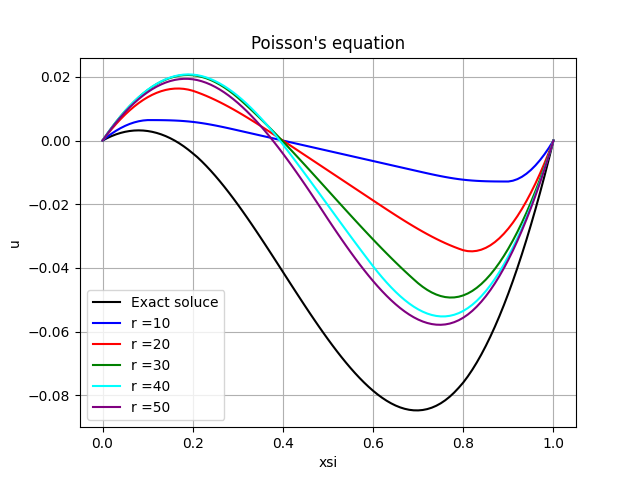
\includegraphics[width=\textwidth]{figures/E1_latex.png}
\caption{Solution of Poisson's equation}
\label{fig:poisson}
\end{figure}

\begin{figure}[h]
\centering
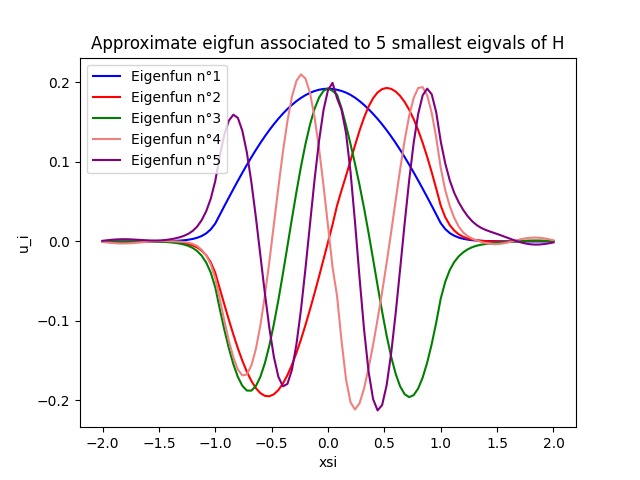
\includegraphics[width=\textwidth]{figures/E2_latex.png}
\caption{Eigenfunctions of Schrödinger's equation}
\label{fig:Schrödinger}
\end{figure}

\end{document}